\chapter{Grundlagen}

Ziel dieser Arbeit ist die Ermittlung optimierter Gebäudeenergiesysteme für den deutschen Wohngebäudebestand.
Hierzu wird in Kapitel \ref{sec:Sektion 21} der Bestand analysiert, um auf dieser Untersuchung aufbauend die nationale Wohngebäudesituation in einigen wenigen, repräsentativen Klassen abzubilden. 
Des Weiteren wird in \ref{sec:Sektion 22} die historische Entwicklung der Gebäudehülle im Neubauzustand betrachtet und in \ref{sec:Sektion 23} die Abweichungen des Neubauzustandes durch Sanierung erläutert. Daraus werden Zeiträume der Baualtersklassen mit ähnlichen Baustoffen und Dämmdicken zusammengefasst. 
Kapitel \ref{sec:Sektion 24} stellt Förderprogramme zum Anreiz energetischer Sanierung vor.
Weiterhin werden in Kapitel Kapitel \ref{sec:Sektion 31} und \ref{sec:Sektion 32} Arten der mathematischen Optimierung sowie das im Rahmen dieser Arbeit erweiterte Optimierungsprogramm vorgestellt und in Kapitel \ref{sec:Sektion 33} die Grundlagen der Lüftungswärmeverlusten in Wohngebäuden. 

\section{Deutscher Wohngebäudebestand}
\label{sec:Sektion 21}

Zunächst wird der Wohngebäudebestand hinsichtlich Alter und Größe ausgewertet.
Als Daten werden die Statistiken des Zensus 2011, einer nationalen statistischen Erhebung von privaten Haushalten, betrachtet. 
Besagte Statistiken werden in verschiedenen wissenschaftlichen Untersuchungen des Instituts für Wohnen und Umwelt GmbH (IWU) ausgewertet und evaluiert.
Weiterhin werden für die gebäudetypischen Kennwerte die Typgebäude des europaweiten Projekts \glqq Typology Approach for Building Stock Energy Assessment\grqq\,(TABULA) berücksichtigt. Die nationalen Daten Deutschlands werden durch das IWU erhoben und berechnet.

Nach den 2011 veröffentlichten Zensus Daten besteht der deutsche Wohngebäudebestand aus rund 18.368.000 Gebäuden mit 39.432.000 Wohnungen \cite{.2015}.
Wie in Abbildung \ref{fig: Abbildung211} zu erkennen ist, prägt den deutschen Wohngebäudebestand einen Boom in der Nachkriegszeit. 
So wurden in den Jahren von 1949 bis 1978 etwa 7,2 Millionen Häuser errichtet. Diese Klasse allein bildet \mbox{38 \%} der deutschen Wohngebäude ab. 
Mit circa 2,7 Millionen Gebäuden und einem Anteil von etwa \mbox{14 \%} bilden die vor 1919 fertiggestellten Wohnobjekte den zweitgrößten Anteil, sowie die Häuser mit Baualter zwischen 1919 und 1948 mit knapp \mbox{12 \%} die drittgrößte Gruppe.
Folglich sind knapp zwei Drittel der deutschen Wohngebäude vor 1978 erbaut worden.
Eine weitere relevante Klasse beschreiben mit fast \mbox{10 \%} die von 1979 bis 1986 geschaffenen Wohnbauten. 
Zusammen mit den drei Klassen \mbox{1987 - 1990,} \mbox{1991 - 1995} und \mbox{1996 - 2000} werden  durch diese vier Gruppen mehr als ein Viertel des Wohngebäudebestandes in Deutschland abgebildet.
Im Gegensatz zu den zuvor genannten Gruppen stellen die nach der Jahrtausendwende konstruierten Häuser mit unter \mbox{10 \%} und nur 1,6 Millionen Häusern einen relativ kleinen Anteil des nationalen Bestandes dar. 

Es sei noch zu erwähnen, dass in dieser Betrachtung den Mikrozensus-Klassen gefolgt wird. 
Diese sind explizit keine gleich langen Zeitintervalle, sondern \glqq orientieren sich an historischen Einschnitten, den Zeitpunkten statistischer Erhebungen und den Veränderungen der wärmetechnisch relevanten Bauvorschriften\grqq \cite{.2015}. 
So beschreibt beispielsweise das relativ kurze Zeitintervall von 1979 bis 1983 den Zeitraum zwischen erster und zweiter Wärmeschutzverordnung, auf welche in Kapitel \ref{sec:Sektion 22} noch näher eingegangen wird.

\begin{figure}[H]
	\centering
		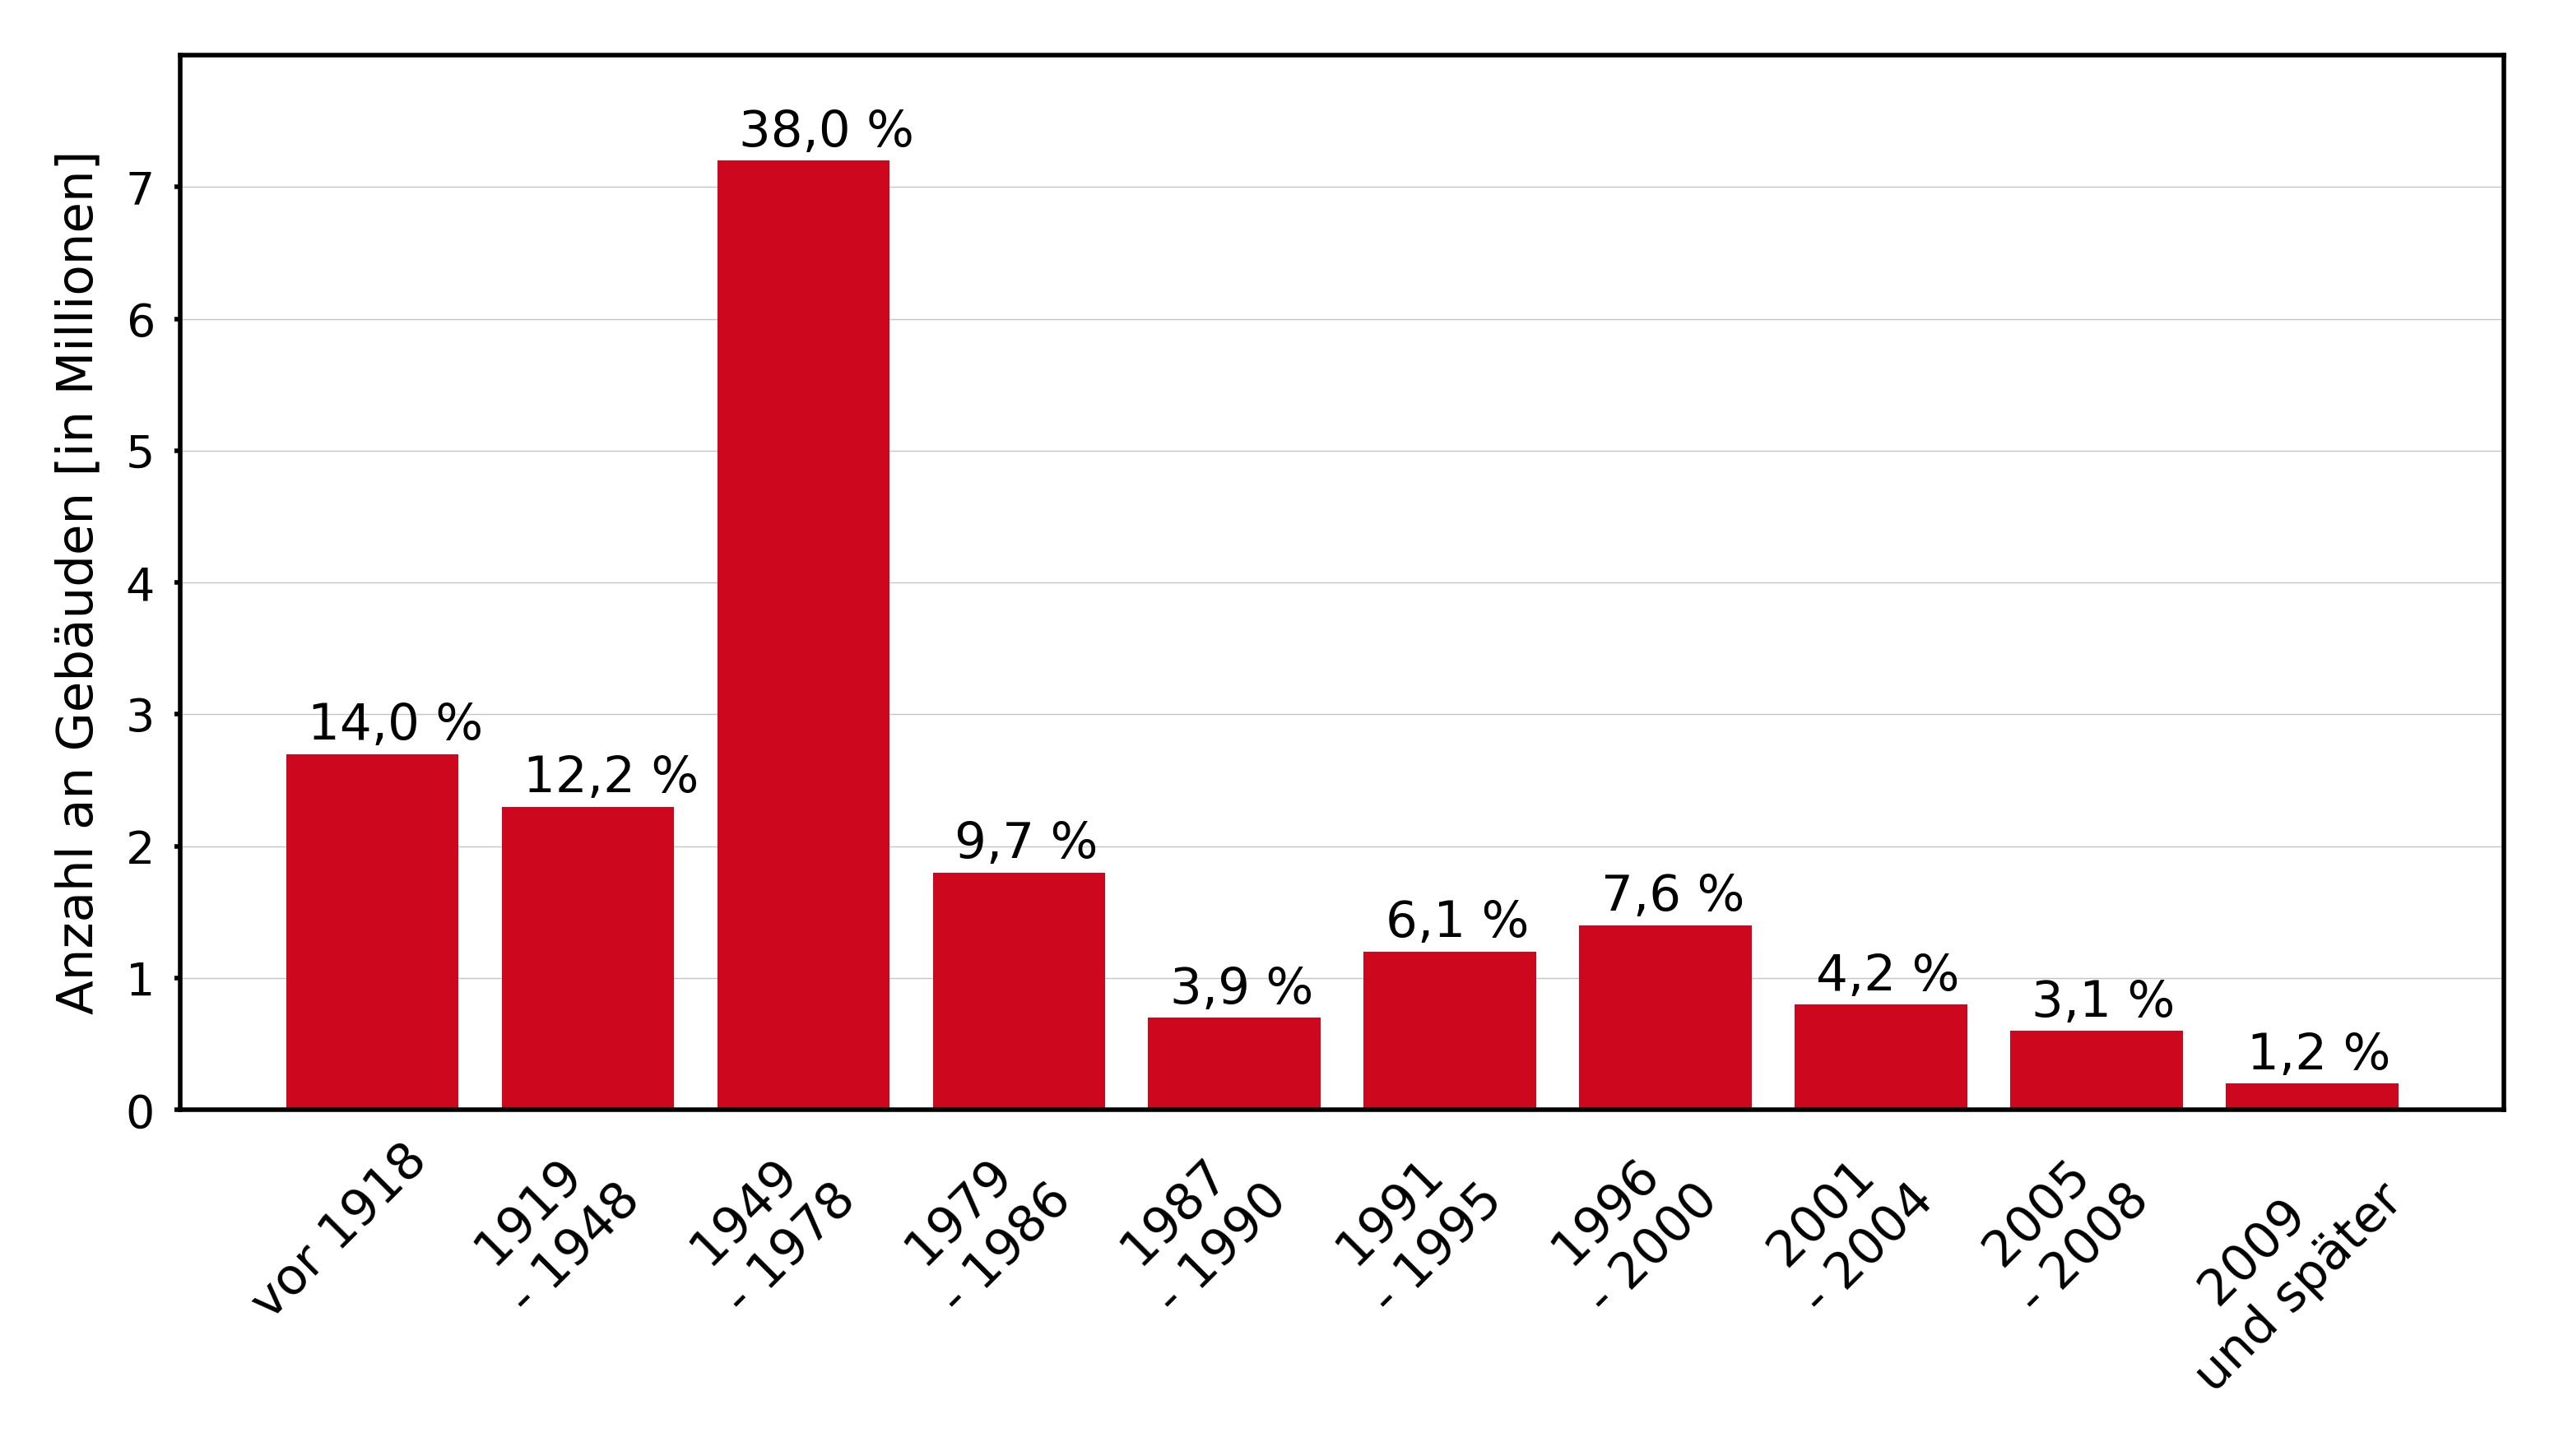
\includegraphics{Pictures/GebaeudeAlterDiagramm.jpg}
	\caption{Errichtete Wohngebäude nach Mikrozensus-Klassen sowie deren Anteil am Gebäudebestand [in \%] \cite{StatistischeAmterdesBundesundderLander.2014}}
	\label{fig: Abbildung211} 
\end{figure}

Eine weitere Unterteilung des Wohngebäudebestandes erhält man bei der Betrachtung der Anzahl an Wohneinheiten im Gebäude. 
Hierbei setzt sich der Bestand zu zwei Dritteln aus Wohngebäuden mit nur einer Wohnung zusammen. 
Weitere \mbox{17 \%} bilden Gebäude mit zwei Wohnungen, während die Gebäudeklasse mit \mbox{3 - 6 Wohnungen} mit \mbox{12 \%} vertreten ist. 
Die größeren Gebäude mit \mbox{7 - 12 Wohnungen} sowie mit 13 und mehr Wohnungen sind anteilig am Gebäudebestand mit jeweils \mbox{5 \%} und \mbox{1 \%} relativ kleine Gruppen. 
Allerdings gelten letztere nur bei einer Gebäudebetrachtung als weniger relevant, da sie bei einer Anschauung der Wohneinheiten logischerweise mit größeren Faktoren im Vergleich zu Einfamilienhäusern einhergehen. \cite{StatistischeAmterdesBundesundderLander.2014b}

In Abbildung \ref{fig: Abbildung212} sind die Anzahl der Wohneinheiten für die drei Baualtersklassen älter als 1978, \mbox{1979 - 1994} und \mbox{1995 - 2009} sowie deren Anteil an allen Wohneinheiten bis Baujahr 2009 des Gebäudebestandes dargestellt. 
In Anlehnung an den vorherigen Abschnitt werden Gebäude mit bis zu 2 Wohnungen als Ein- und Zweifamilienhäuser zusammengefasst und mit EFH abgekürzt
Wohngebäude mit 3 oder mehr Wohnungen werden als Mehrfamilienhäuser mit der Abkürzung MFH gebündelt. 

Auffallend ist wiederum der enorme Anteil der Gebäude mit Baualter älter als 1978. 
Hier zählen die Mehrfamilienhäusern mit 14,8 Millionen Wohnungen und einem Anteil aller bis 2009 errichteten Wohneinheiten von \mbox{38 \%} zur größten Gruppe. 
Mit 12,5 Millionen Wohnungen und einem Anteil von 32\,\% entfällt die zweitgrößte Klasse auf die Einfamilienhäuser mit Baujahr älter 1978.
Ähnlich wie zuvor bei der Gebäudebetrachtung wurden somit auch mehr als zwei Drittel aller Wohnungen vor 1978 erbaut.

\begin{figure}[H]
	\centering
		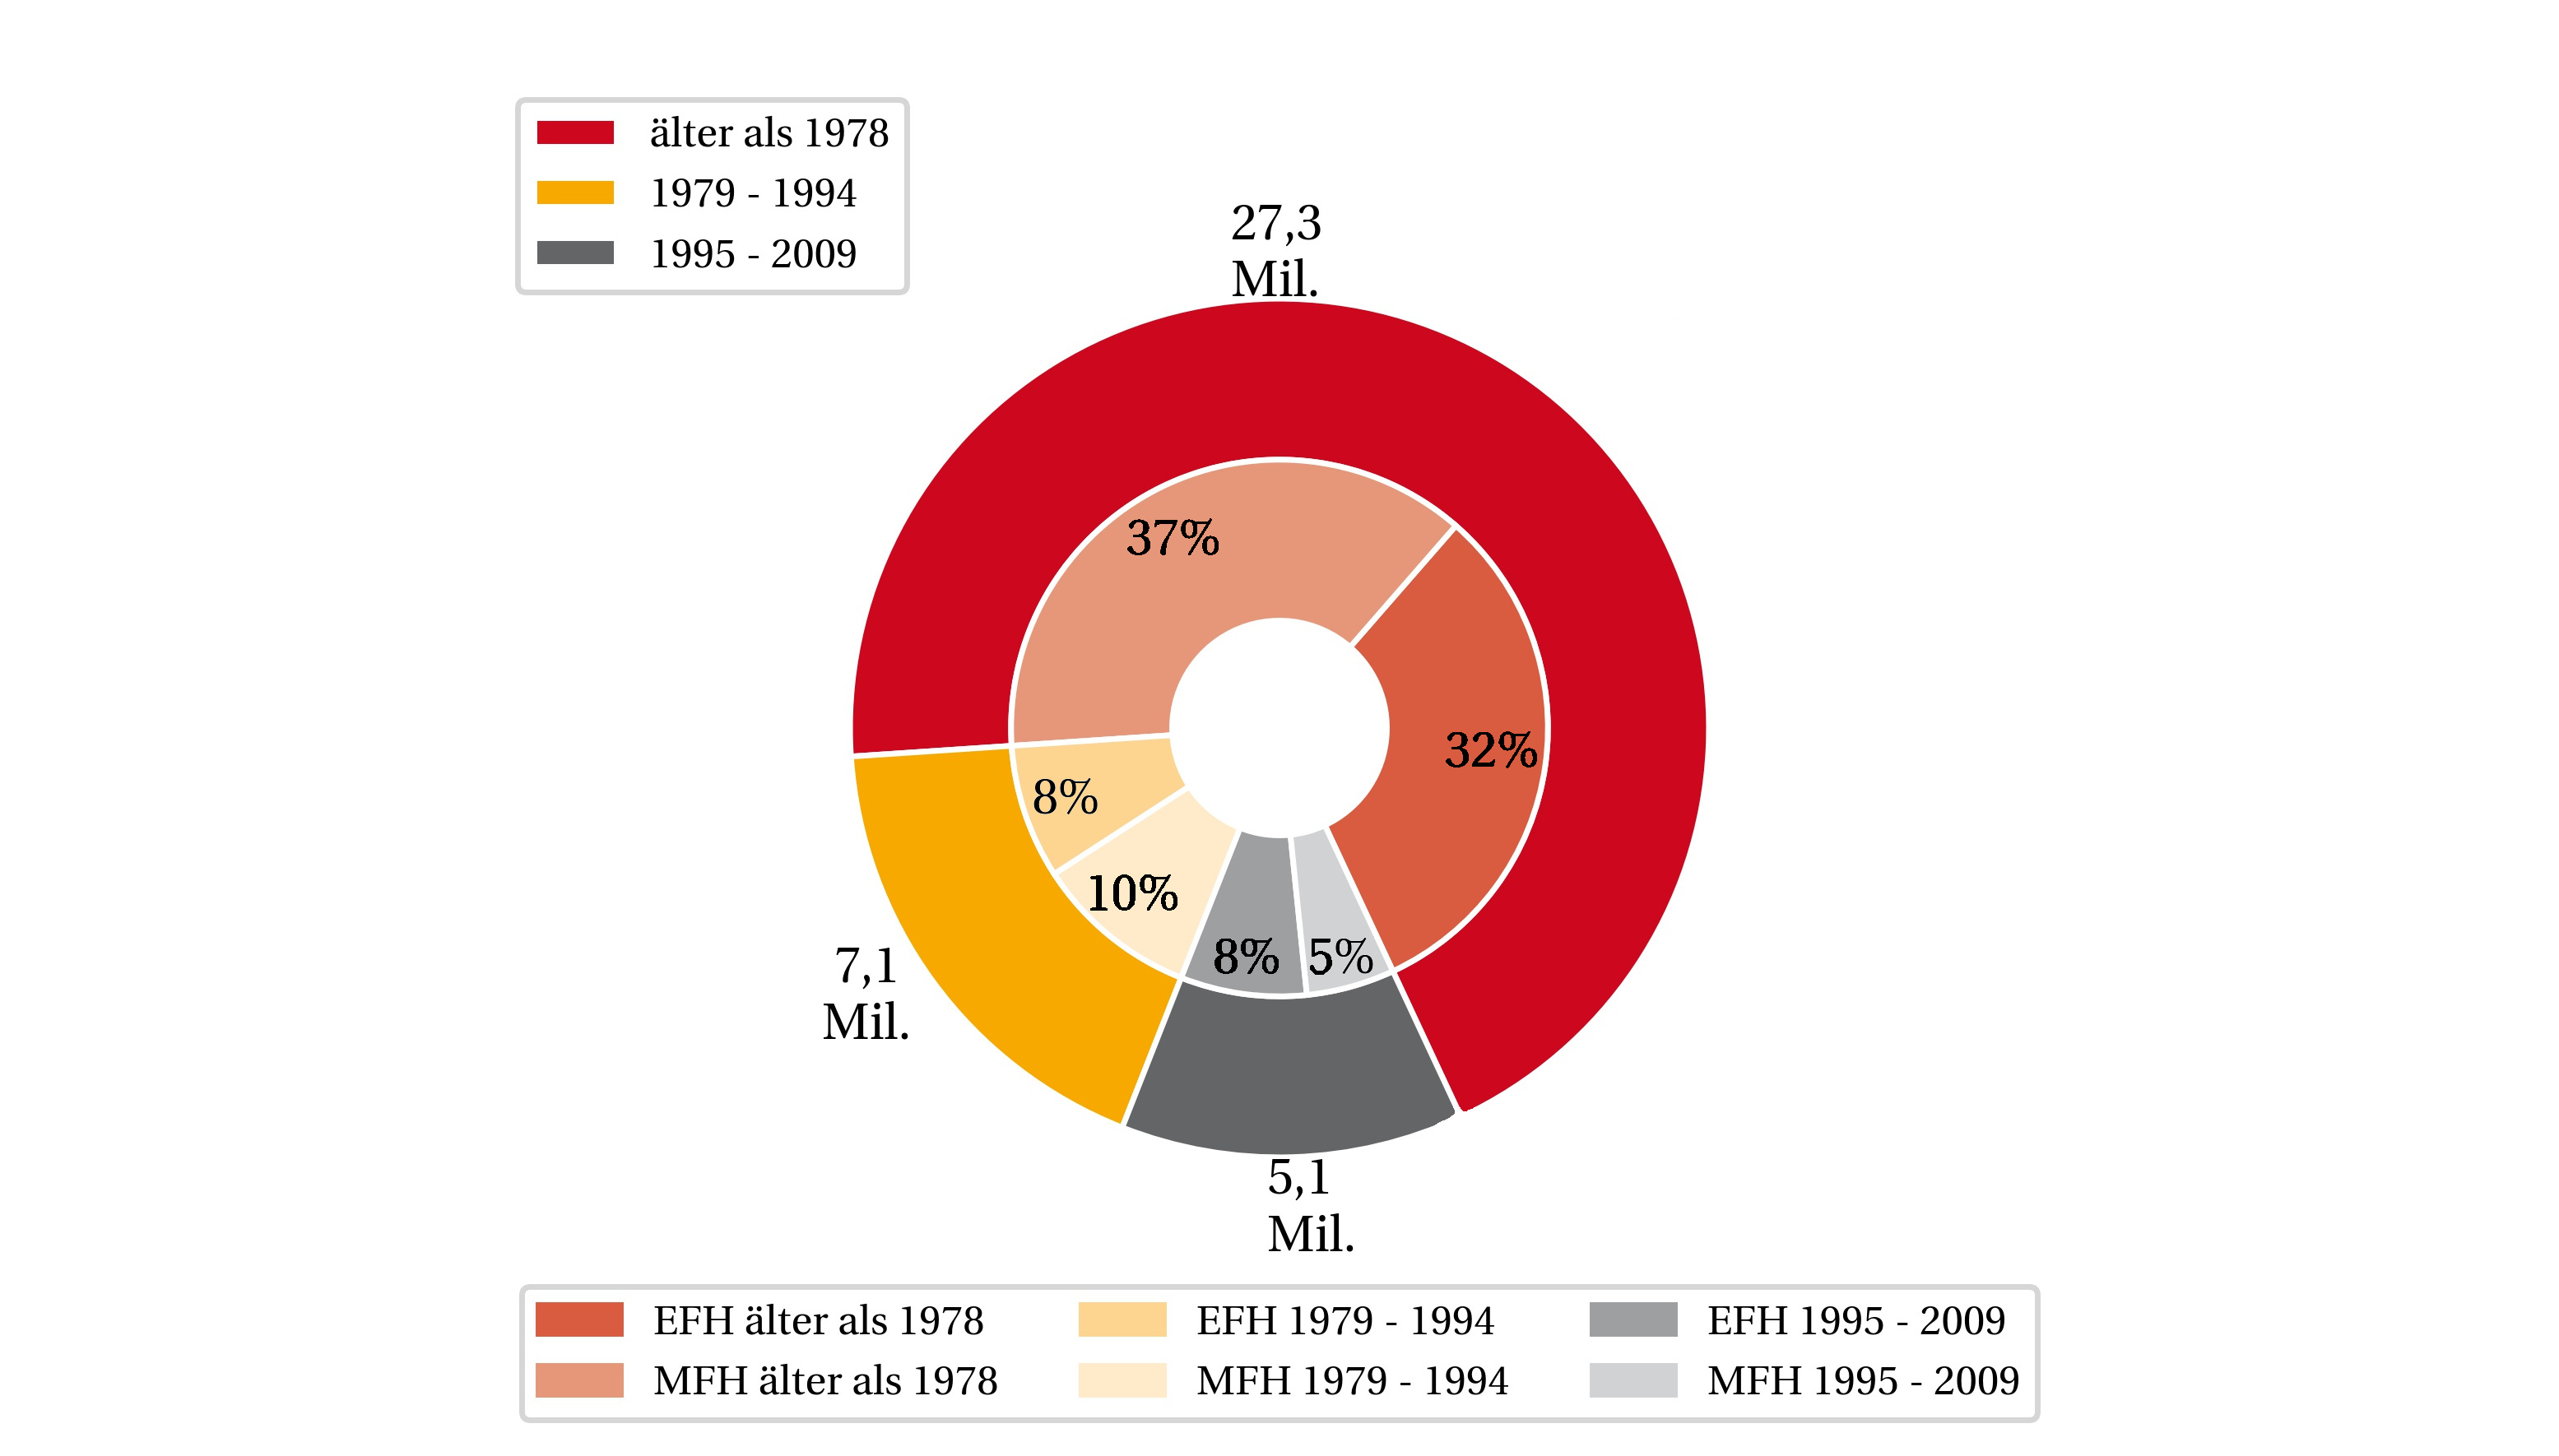
\includegraphics{Pictures/GebaeudeGroesse.jpg}
	\caption{Anzahl an Wohneinheiten bei Ein- und Zweifamilienhäuser (EFH) und Mehrfamilienhäuser (MFH) sowie deren relativer Anteil [in \%] nach Baualtersklassen. \cite{StatistischeAmterdesBundesundderLander.2014b}}
	\label{fig: Abbildung212} 
\end{figure}

Eine detailliertere Gliederung der Gebäudetypen ist in Tabelle \ref{tab: TabelleA0} zu finden. 
Hier wurden die Anzahl der Wohneinheiten nach Baualtersklasse und Gebäudetyp eingeteilt. 
Zu den zuvor beschriebenen Ein- und Mehrfamilienhäusern sind in der Tabelle außerdem die Klassen der Reihenhäusern , großen Mehrfamilienhäuser sowie Hochhäusern zu ermitteln. 
Weiter lassen sich die Anzahl der Wohnungen für diverse Gebäudearten in neuen Bundesländern ablesen.

Zusammenfassend lassen sich folgende Punkte bei der statistischen Betrachtung des deutschen Gebäudebestandes festhalten:

\begin{itemize}
	\item $\nicefrac{2}{3}$ aller Gebäude und Wohnungen des Bestandes wurden vor der 1. Wärmeschutzverordnung 1978 errichtet.
	\item Bei einer Betrachtung der Wohneinheiten halbiert sich der Bestand in Gebäude mit einer oder zwei Wohnungen (47\,\%) und drei oder mehr Wohnungen (53\,\%).
	\item Gebäude, die nach der Jahrtausendwende gebaut wurden, bilden keinen signifikanten Anteil des Bestandes.
\end{itemize}

\section{Historische Entwicklung der Gebäudehülle}
\label{sec:Sektion 22}

Nachdem das vorherige Kapitel den Gebäudebestand nach Alter und Größe beschreibt, werden nun die zu den jeweiligen Gebäudealtern zugehörigen Baustoffe und Dämmeigenschaften vorgestellt. 
Hierzu wird zwischen der Isolierung verschiedener Gebäudebauteilen, die im Kontakt mit der Umgebung oder einem unbeheizten Raum stehen, unterschieden. 
Neben Möglichkeiten zur Dämmung des Daches beziehungsweise der obersten Geschossdecke und der Außenwand werden zudem die Dämmung des Bodens betrachtet.
Weiterhin wird auf den Verglasungsstandard verschiedener Epochen eingegangen.

Ein wichtiger Kennwert zur energetischen Bewertung eines Gebäudes und einzelner Gebäudekomponenten beschreibt der U-Wert.
Hierbei handelt es sich um den Wärmeübergangskoeffizienten, welcher den Wärmestrom durch 1\,m² Bauteilfläche bei 1\,K Temperaturdifferenz beschreibt. 
Berechnet wird dieser als Kehrwert des Wärmedurchgangswiderstand R\(_T\). 
Der U-Wert ist definiert als
\begin{equation}
\label{eq:Gleichung221}
U = \frac{1}{R_T}  \qquad \text{in} \ \ \frac{W}{m^2 \cdot K} 
\end{equation}
wobei mit
\begin{equation}
\label{eq:Gleichung222}
R_T = \sum \limits_{i} \frac{d_i}{\lambda_i}	
\end{equation}				%Muss ich da innere, äußere Schicht unterscheiden?
der Wärmedurchgangswiderstand als Verhältnis der Dämmstoffdicke d\(_i\) einer Dämmschicht i und der Wärmeleitfähigkeit \(\lambda_i\) des Baustoffes der Schicht i beschrieben wird. 

Für transparente Bauteile und somit explizit für Fenster variiert die Berechnung des Wärmedurchgangskoeffizienten U\(_w\):
\begin{equation}
\label{eq:Gleichung223}
U_w = \frac{A_g \cdot U_g + A_f \cdot U_f + l_g \cdot \psi_g}{A_g + A_f}  \qquad \text{in} \ \ \frac{W}{m^2 \cdot K}
\end{equation}
Hierbei beschreiben A\(_f\) den Flächenanteil des Fensterrahmens und A\(_g\) die Glasfläche. Ferner sind U\(_g\) und U\(_f\) die Wärmeübergangskoeffizienten der Verglasung (Index g) und des Fensterrahmens (Index f). 
Außerdem werden Wärmebrückenbildungen des Glasrandverbundes mit der Multiplikation des \(\psi\)-Wertes mit der Gesamtumfangsfläche der Verglasung l\(_g\) berücksichtigt. \cite{Laasch.2013}
%Wärmebrücken erklären?

Aus den Definitionen der U-Werte und des Wärmedurchgangswiderstandes lässt sich leicht erkennen, dass die Transmissionswärmeverluste eines Gebäudes stark von der Dicke und den Dämmeigenschaften des Dämmmaterials abhängen. 
Hierbei lassen sich historische Unterscheidungen treffen.

Die drei TABULA-Klassen \mbox{vor 1918}, \mbox{1919 - 1948} sowie \mbox{1949 - 1957} umfassen die Epochen der Gründerzeit, der Zwischenkriegszeit, den beiden Weltkriegen sowie der Nachkriegszeit. 
Wie in Kapitel \ref{sec:Sektion 21} bereits dargelegt, prägen die Nachkriegsjahre einen schnellen Wiederaufbau, in dem vor allem mit Trümmern neue Gebäude errichtet wurde. 
Auch in dem Zeitraum \mbox{vor 1918} kam es im Rahmen der Ausdehnung der Städte zu zahlreichen neuen Konstruktionen. 
Aus Tabelle \ref{tab: TabelleA1} lässt sich erkennen, dass sich die Wärmeübergangskoeffizienten für die Gebäudetypen der Einfamilien- und Mehrfamilienhaus in diesen Jahren jeweils stark ähneln. 
Dies ergibt sich auch aus der Darstellung der Geschichte des Dämmstandards von Eicke-Henning. %hier schon zitat?
Hier wird festgehalten, dass sich bis zum Jahr 1957 die Dämmindustrie und der Hochbau im Rahmen der Industrialisierung zwar weiterentwickelte, es allerdings dennoch keinen Wandel im Hinblick auf Wärmeschutz gab.
So wurde bevorzugt günstig gebaut und die damit verbunden erhöhten Heizkosten in Kauf genommen oder durch niedrige Raumtemperaturen kompensiert.
Die im Jahr 1952 eingeführte DIN 4108 verkörperte zwar den ersten Ansatz Wärmeschutz normativ zu regulieren, jedoch konnte sie zu keiner Veränderung der energetischen Bauweise führen. 
Trotz deren Name \glqq Wärmeschutz im Hochbau\grqq\,beinhaltet die Norm nur einen Mindestwärmeschutz zur Vermeidung bauphysikalischer Schäden durch Schimmelbildung.
Als Standard dieser Jahre galt das 38\,cm dicke Vollziegel-Mauerwerk, Böden und Dächer ohne Dämmung sowie die Einscheiben-Verglasung. \cite{EickeHenning.2011}

In den folgenden Jahren von \mbox{1958 - 1968} sowie \mbox{1969 - 1978} kam es zu keinen normativen Änderungen des Wärmeschutzes. 
Dennoch kann durch einen Wandel der Baustoffwahl eine Verbesserung der U-Werte beobachtet werden. 
So verschwand der Vollziegel langsam vom Markt und wurde durch Hochlochziegeln oder Hohlblocksteinen substituiert.
Weiter wurden vermehrt Trittschalldämmungen in Böden und Dächer installiert. 
Trotz deren primären Zweckes der Lärmvermeidung erzielten diese dünnen Dämmschichten von \mbox{1 - 4 cm} Dämmstärke eine Verbesserung der Wärmedurchgangskoeffizienten der zuvor genannten Bauteile.
Ab 1965 erreichten vorgefertigte Betonteile mit einem \mbox{3 - 6 cm} dicken Dämmkern zudem einen besseren Wärmeschutz.
Bezüglich der Fenster wurde in diesen Jahren keine Veränderung geschaffen, so dass weiterhin die Einscheiben-Verglasung die Konvention bildete. \cite{EickeHenning.2011}

Nach der Ölkrise von 1974 rückte die Bedeutung des ressourcenschonenden Bauens beziehungsweise Betriebes von Gebäuden in den Vordergrund. 
Der Gesetzgeber verabschiedete am 11. August 1977 mit der 1. Wärmeschutzverordnung, im Folgenden mit WschV abgekürzt, erstmalig eine Verordnung, in der ein Standard zur Minimierung des Heizwärmebedarfs festgelegt wurde. 
In Folge der 1. WschV verbesserte sich die Dämmeigenschaften der Bauten mit Baujahr \mbox{1979 - 1983}.
So lässt sich bei den TABULA Einfamilienhäuser dieser Jahrgänge feststellen, dass sowohl das Dach eine 8\,cm als auch der Boden eine 4\,cm dicke Dämmschicht besitzen. 
Dadurch konnten U-Werte von 0,5\,\(\frac{W}{m^2 \cdot K} \) für das Dach sowie 0,65\,\(\frac{W}{m^2 \cdot K} \) für den Boden erreicht werden (s. Tabelle \ref{tab: TabelleA1}).
Weiterhin wurde durch die Verordnung vorgeschrieben, dass \glqq außenliegende Fenster und Fenstertüren von beheizten Räumen (...) mindestens mit Isolier- und Doppelverglasung auszuführen (sind)\grqq \cite{Bundesregierung.1977}.
Somit ermöglichte die 1. WschV eine Verbesserung des energetischen Standards der Wohngebäuden. 
Allerdings stellten die ersten normativen Anforderungen an die Gebäudehülle aus heutiger Sicht nur einen Zwischenschritt hin zu einem energetisch sinnvollen Reglement dar.
Als Beispiel hierfür ist die Anforderung an Fenster zu nennen. 
Für diese wurde in der 1. WschV festgelegt, dass ein U-Wert von 3,5\,\(\frac{W}{m^2 \cdot K} \) nicht überschritten werden darf \cite{Bundesregierung.1977}.
Nach heutigem Standard der Energieeinsparverordnung 2016, die im Folgenden noch weiter erläutert wird, sind für die Fenster im Neubau U\(_w\)-Werte kleiner 1,3\,\(\frac{W}{m^2 \cdot K} \) einzuhalten.
Bei diesem Vergleich ist auch noch festzuhalten, dass es sich bei der Vorgabe zum U-Wert der 1. WschV um den U\(_g\)-Wert handelt, der nur den Wärmedurchgang durch die Verglasung beschreibt und somit im Gegensatz zu U\(_w\) weder den Wärmeübergang durch den Rahmen noch die Wärmebrückenbildung beachtet. 
Daher liegt der von TABULA ermittelte U\(_w\)-Wert für das Einfamilien-Typgebäudenfenster der Jahre \mbox{1979 - 1983} aufgrund dessen energetisch schlechten Metallrahmens mit 4,3\,\(\frac{W}{m^2 \cdot K} \) höher als der U\(_g\)-Normwert der 1. WschV. \cite{EickeHenning.2011} 

Einen weiteren Schritt hin zu einem besseren Wärmeschutz des Gebäudebestandes markiert die 1982 beschlossene und 1984 in Kraft getretene 2. WschV, die sich auf den Wärmeschutz der Gebäude mit Baujahr \mbox{1984 - 1994} auswirkte.
Nach Eicke-Henning kann sich \glqq das Niveau von 1984 (...) mit 2-Scheiben-Isolierverglasung, 30\,cm dicken porosierten Außenwänden (...), 8-9\,cm Wärmedämmung im Dach und 4\,cm Kellerdämmung beschreiben (lassen) \grqq\,\cite{EickeHenning.2011}.
Wie sich aus Tabelle \ref{tab: TabelleA1} lesen lässt, führten die Maßnahmen der 2.\,WschV zu einem durchgehend besseren Verhalten der Bauteile gegenüber Transmissionswärmeverlusten. 
Im Bezug auf die Anforderung der Fensterflächen ergab sich zwar eine Verbesserung im Vergleich zur 1.\,WschV auf \(U_{g, max} = 3,1\,\frac{W}{m^2 \cdot K} \), allerdings blieb die im vorangegangenen Abschnitt diskutierte Problematik des \(U_g\)-Wertes erhalten.
Des Weiteren definierte die 2. WschV Anforderungen an \glqq Bauliche Änderungen bestehender Gebäude\grqq.
Daraus folgte, dass bei Gebäudeerweiterungen oder Umbaumaßnahmen das betroffene Bauteil den geforderten energetischen Neubaustandard erfüllen musste.

Einen Paradigmenwechsel des Wärmeschutzes kennzeichnet die 3.\,Verordnung über einen energiesparenden Wärmeschutz bei Gebäuden von 1995.
Im Gegensatz zu den zuvor vorgestellten Verordnungen begrenzte die 3.\,WschV nicht nur die U-Werte der Bestandteile der Gebäudehülle, sondern beschränkte zudem den Jahres-Heizwärmebedarf.
Als Folge der neuen Verordnung erhielten die Bauteile im Vergleich zur 2. WschV \mbox{4 - 6 cm} mehr Dämmdicke. 
Außerdem wurde durch die erhöhten Anforderungen an die Verglasung die Zweischeiben-Wärmeschutzverglasung der Neubaustandard.
Aufgrund dieser Maßnahmen konnten die U-Werte der Gebäude mit Baujahr \mbox{1995 - 2001} signifikant gesenkt werden.
Besonders die bessere Verglasung mit wärmetechnisch besseren Rahmen erzielte eine Verbesserung des \(U_g\)-Wertes von \mbox{3 - 3,2 \(\frac{W}{m^2 \cdot K} \)} auf 1,9\,\(\frac{W}{m^2 \cdot K}\).

Die zum 01. Februar 2002 in Kraft getretene Energieeinsparverordnung (EnEV) legte die zuvor genannte 3. WschV sowie die Heizungsanlagenverordnung zusammen. 
Somit wurden alle Anforderungen an den Energieverbrauch eines Gebäudes in einer Verordnung gebündelt.
Anstelle der Begrenzung des Jahres-Heizwärmebedarfes, wie im Abschnitt zuvor, wurde der Jahres-Primärenergiebedarf sowie der flächenspezifische Transmissionswärmeverlust (H\(_t'\)) limitiert.
Obwohl nicht explizit strengere Regulationen an die Gebäudehülle formuliert wurden, konnte durch die Restriktion von \(H_t'\) ein Absinken der Wärmedurchgangskoeffizienten aufgrund dickerer Dämmstärken erzielt werden.
Nach Tabelle \ref{tab: TabelleA1} sank der U-Wert des Zeitraumes \mbox{2002 - 2009} für alle Komponenten der Gebäudehülle im Rahmen der \mbox{EnEV 2002}.
Außerdem setzte die Verordnung striktere Anforderungen an den Altbaubestand. 
So mussten vor dem 01.10.1978 eingebaute Heizkessel mit flüssigem oder gasförmigen Brennstoff ersetzt werden, ungedämmte und zugängliche Wärmeverteilungs- und Warmwasserleitungen nachgedämmt werden sowie nicht begehbar, zugängliche oberste Geschossdecken auf einen U-Wert von 0,3 \(\frac{W}{m^2 \cdot K} \) gedämmt werden.

Auf die EnEV 2002 folgten 2004 sowie 2007 Novellierungen.
Diese stellten keine Verschärfung der energetischen Anforderungen nach EnEV 2002 dar, sondern galten der Beseitigung juristischer Problematiken sowie der Einführung des Energieausweises für Bestandsgebäude \cite{Wild.2015}.
Eine solche Verschärfung wurde hingegen durch die EnEV 2009 vollzogen.
Zum einen wurde die Berechnung des Jahres-Primärenergiebedarfes umgestaltet.
Das Berechnungsverfahren nach EnEV 2009 bestimmt einen flächenspezifischen Höchstwert des Jahres-Primärenergiebedarfes, welcher durch ein Referenzgebäude gleicher Geometrie, Gebäudenutzfläche und Ausrichtung kalkuliert wird.
Die U-Werte der Referenzgebäudeberechnung wurden für die TABULA-Typgebäude der Baujahre \mbox{2010 - 2015} übernommen und sind in Tabelle \ref{tab: TabelleA1} zu finden.
Zum anderen wurden die Grenzwerte \(H_{t, max}'\) in weniger Kategorien im Vergleich zur EnEV 2002 unterteilt und verschärft.
%EnEV Zitate

\begin{figure}[H]
	\centering
		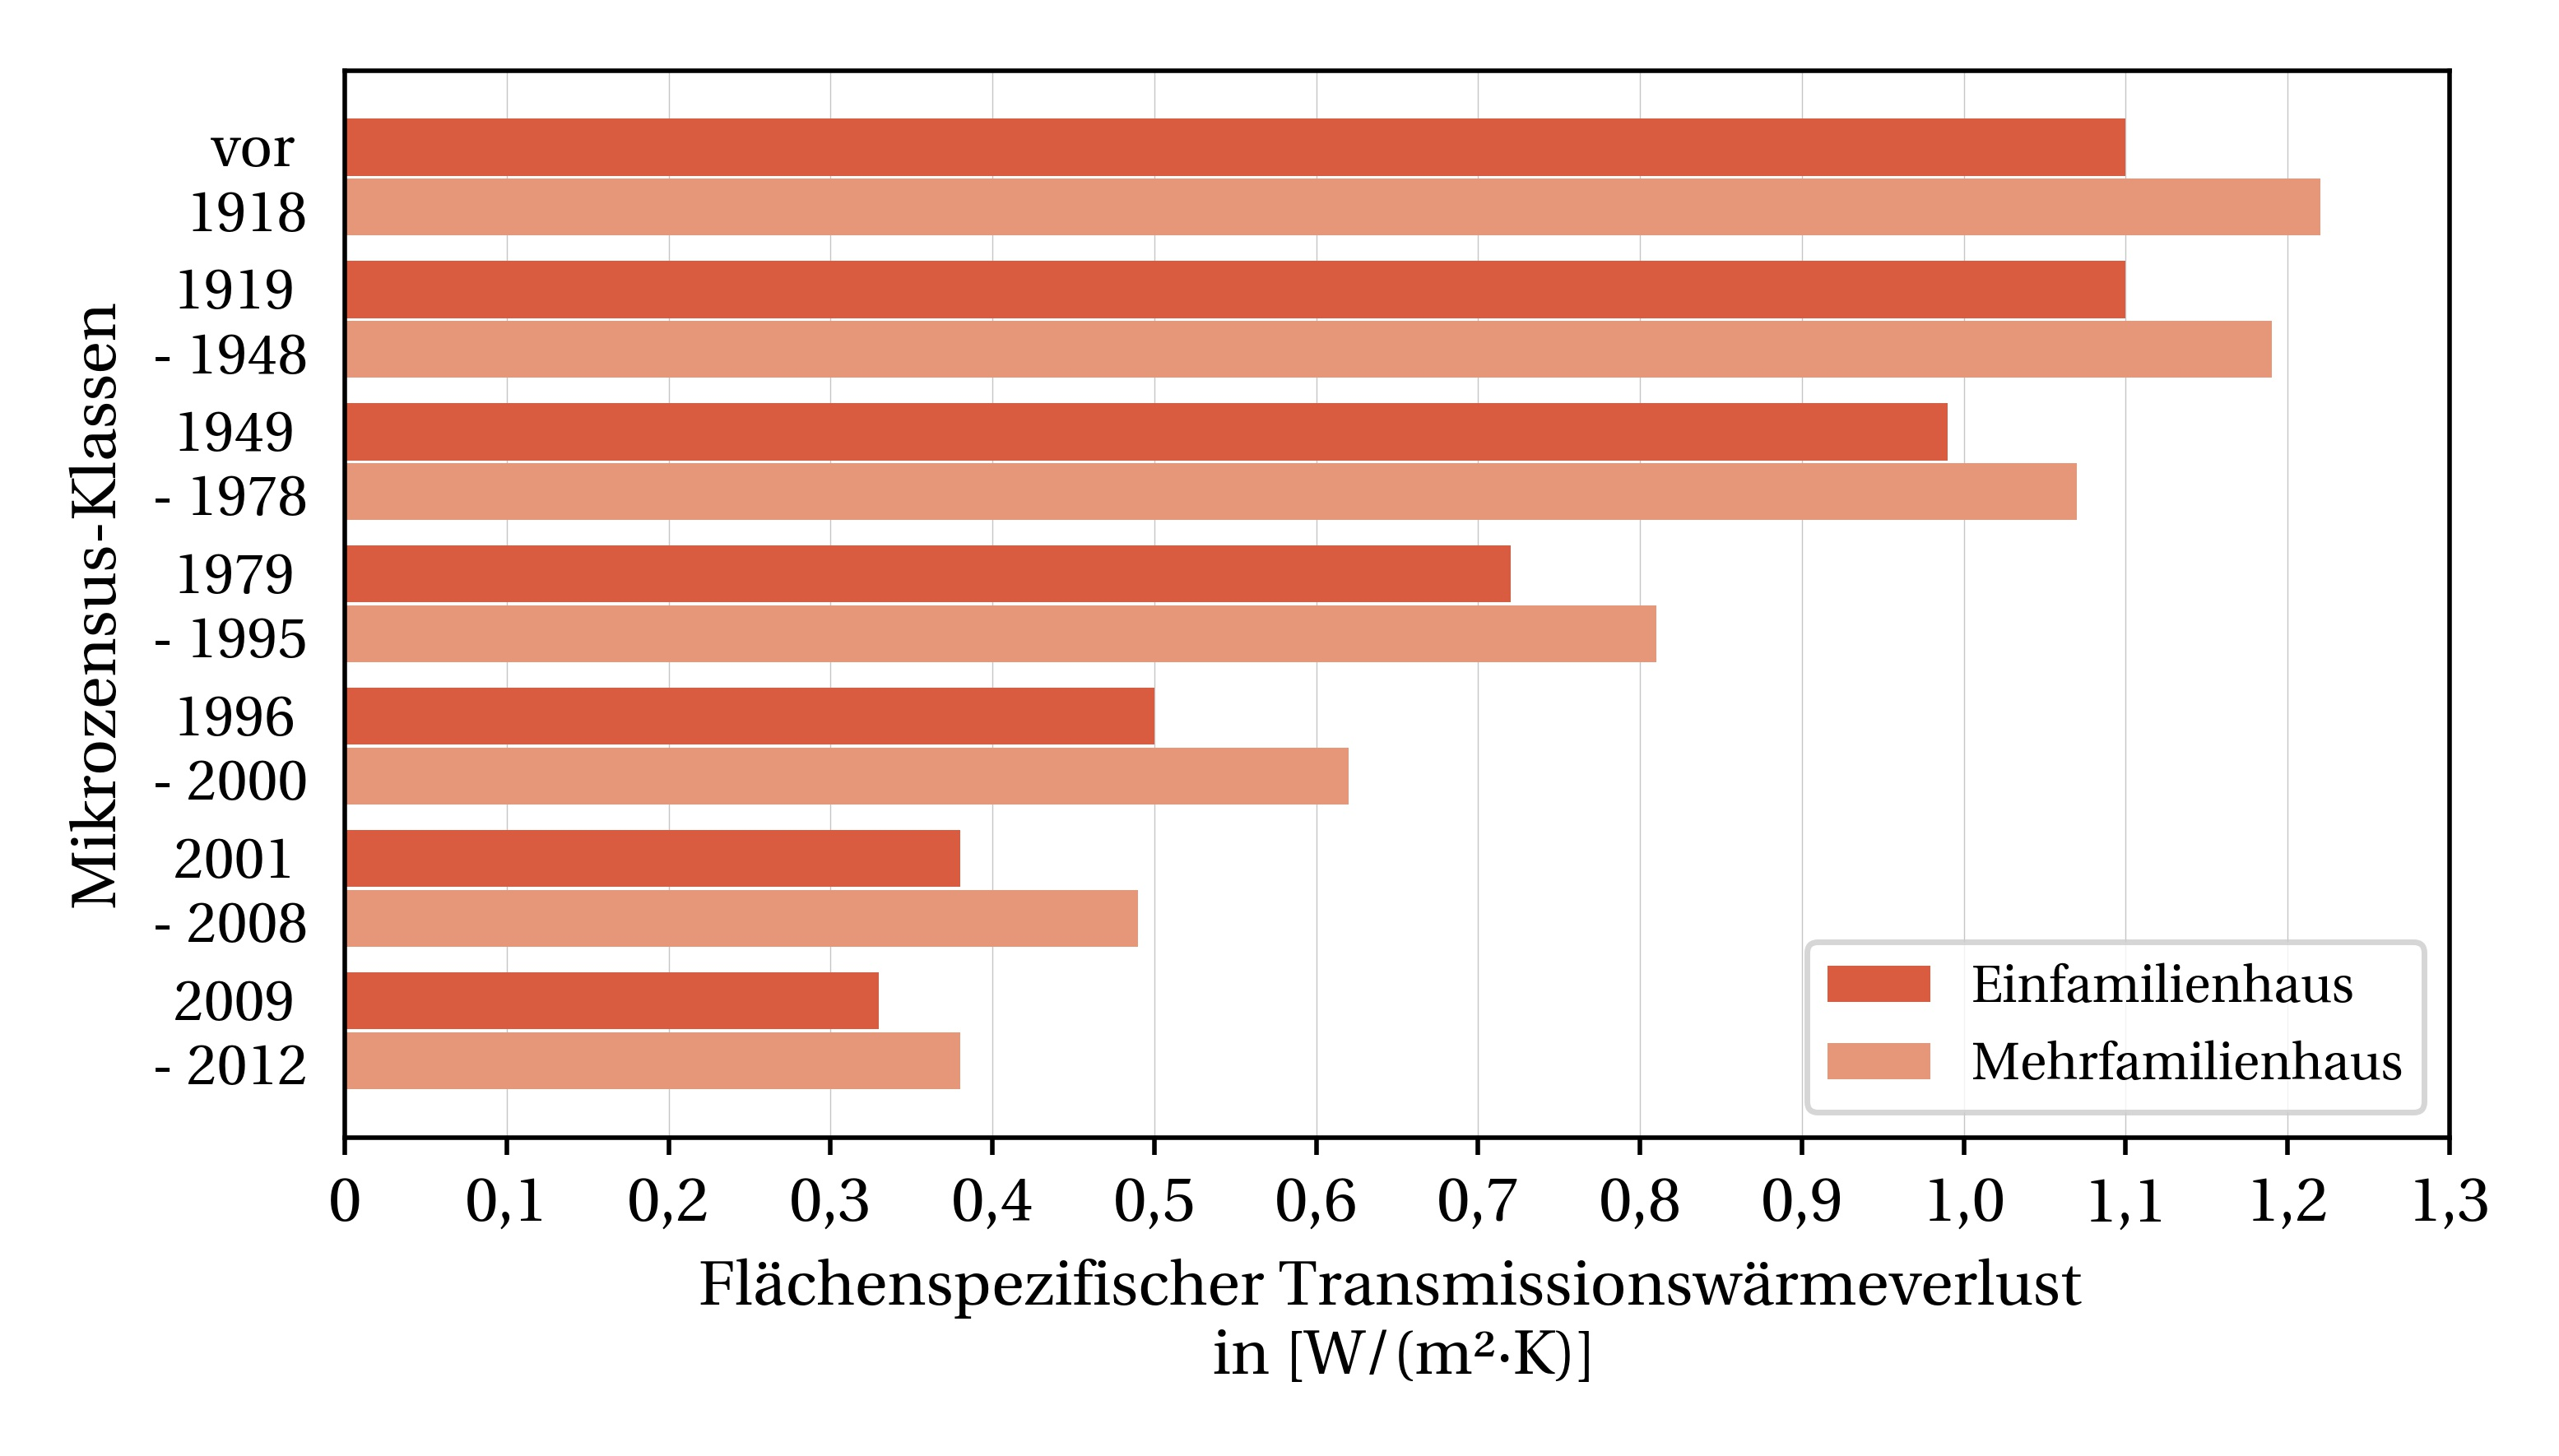
\includegraphics{Pictures/TransmissionswaermekoeffizientBaujahr.jpg}
	\caption{Flächenspezifischer Transmissionswärmeverlust \(H'_t\) nach Baujahr und Gebäudeart. \cite{Bigalke.2016}}
	\label{fig: Abbildung221} 
\end{figure}

Abbildung \ref{fig: Abbildung221} zeigt den flächenspezifischen Transmissionswärmeverlust der Gebäudetypen EInfamilien- sowie Mehrfamilienhaus für verschiedene Baujahre. 
Zu erkennen ist zum einen, dass die Werte der größeren Gebäude immer über denen der Einfamilienhäuser liegen und zum anderen die kontinuierliche Verbesserung im Zuge der energetisch günstigeren Gestaltung der Wohngebäude.
Weiterhin ist festzustellen, dass durch die Wärmeschutz- und Energieeinsparverordnungen der letzten 40 Jahre die flächenspezifische Transmissionswärmeverluste der Neubauten um Vergleich zu einem Altbau um fast 75\,\% gesunken sind.

Zu Tabelle \ref{tab: TabelleA1} ist anzumerken, dass sich auf den Zustand der Bauteile im damaligen Neubau bezogen wird. 
Einzige Ausnahme hierbei bilden die Fenster der Zeiträume bis 1978. 
Für diese charakterisiert die Einscheiben-Verglasung den Einbau-Zustand.
In Kapitel \ref{sec:Sektion 24} wird der Rückgang dieser Fensterart näher erläutert.
%XXXX Zeitstrahl mit Transmissionswärmeverlusten

\section{Sanierungsstand des deutschen Wohngebäudebestandes}
\label{sec:Sektion 23}

In dem vorangegangen Abschnitt wird die Entwicklung der Gebäudehülle aus Wärmeschutztechnischer Sicht vorgestellt. 
Hierbei wird sich auf den Neubauzustand bei Fertigstellung des Gebäudes bezogen.
Dieses Kapitel soll nun die Veränderung des Gebäudebestandes durch energetische Sanierung veranschaulichen.

Abbildung \ref{fig: Abbildung231} zeigt den Anteil der durch nachträgliche Wärmedämmung sanierten Bauteilflächen nach Bauteilen und Gebäudeart.
Zu erkennen ist der große Anteil an sanierter Dachfläche beziehungsweise obere Geschossdeckenfläche.
Dieser liegt für Einfamilien- und Mehrfamilienhäuser annähernd gleich bei etwa 57\,\%.
Folglich wurden mehr als die Hälfte der Dachflächen im Altbau nachträglich gedämmt.
Einen leichten Unterschied zwischen den Gebäudearten ist bei den nachträglich sanierten Außenwänden zu beobachten. 
Bei diesem Bauteil wurden bei den größeren Gebäuden etwas mehr als 31\,\% mit einer besseren Dämmung versehen, wohingegen es bei den Einfamilienhäusern nur etwa ein Viertel waren.
Deutlich weniger Relevanz bei der nachträglichen Dämmung erhielt die Isolierung der Grundplatte beziehungsweise der Kellerdecke. 
Für diese Bauteile wurden bei beiden Gebäudearten nur circa 10\,\% mit einem besseren Wärmeschutz versehen. 

In Abbildung \ref{fig: Abbildung231} fehlen die Angaben zum Sanierungsstand der Fenster.
Hierfür ist die Datenlage der Sanierung schwierig, allerdings bietet das IWU eine Schätzung über den Bestand an Fenstern im Jahre 2015 \cite{Bigalke.2016}.
Tabelle \ref{tab: TabelleA2} gibt verschiedene Verglasungsarten mit deren U\(_g\)-Werten sowie Anzahl und Anteil am gesamten Fensterbestand in Deutschland wieder.
Wie in Gleichung \ref{eq:Gleichung223} dargelegt, beschreibt der U\(_g\)-Wert den Wärmedurchgang durch die Verglasung ohne Berücksichtigung des Fensterrahmens oder der Wärmebrückenbildung.

Obwohl die Einfachverglasung für die Mehrheit des Altbaus den Neubaustandard darstellte, ist deren Anteil am heutigen Fensterbestand mit nur 3\,\% sehr gering. 
Der heutige Bestand der Fenster wird durch unbeschichtetes Isolierglas sowie dem Zweischeiben-Wärmedämmglas dominiert, welche mit respektiv 34\,\% und 47\,\% vertreten sind.
Weiterhin ist zu erkennen, dass das Dreischeiben-Wärmedämmglas bereits 8\,\% des Fensterbestandes bereitstellt, obwohl dieses erst 10 Jahren vor Erhebung der Daten auf den Markt kam.

\begin{figure}[H]
	\centering
		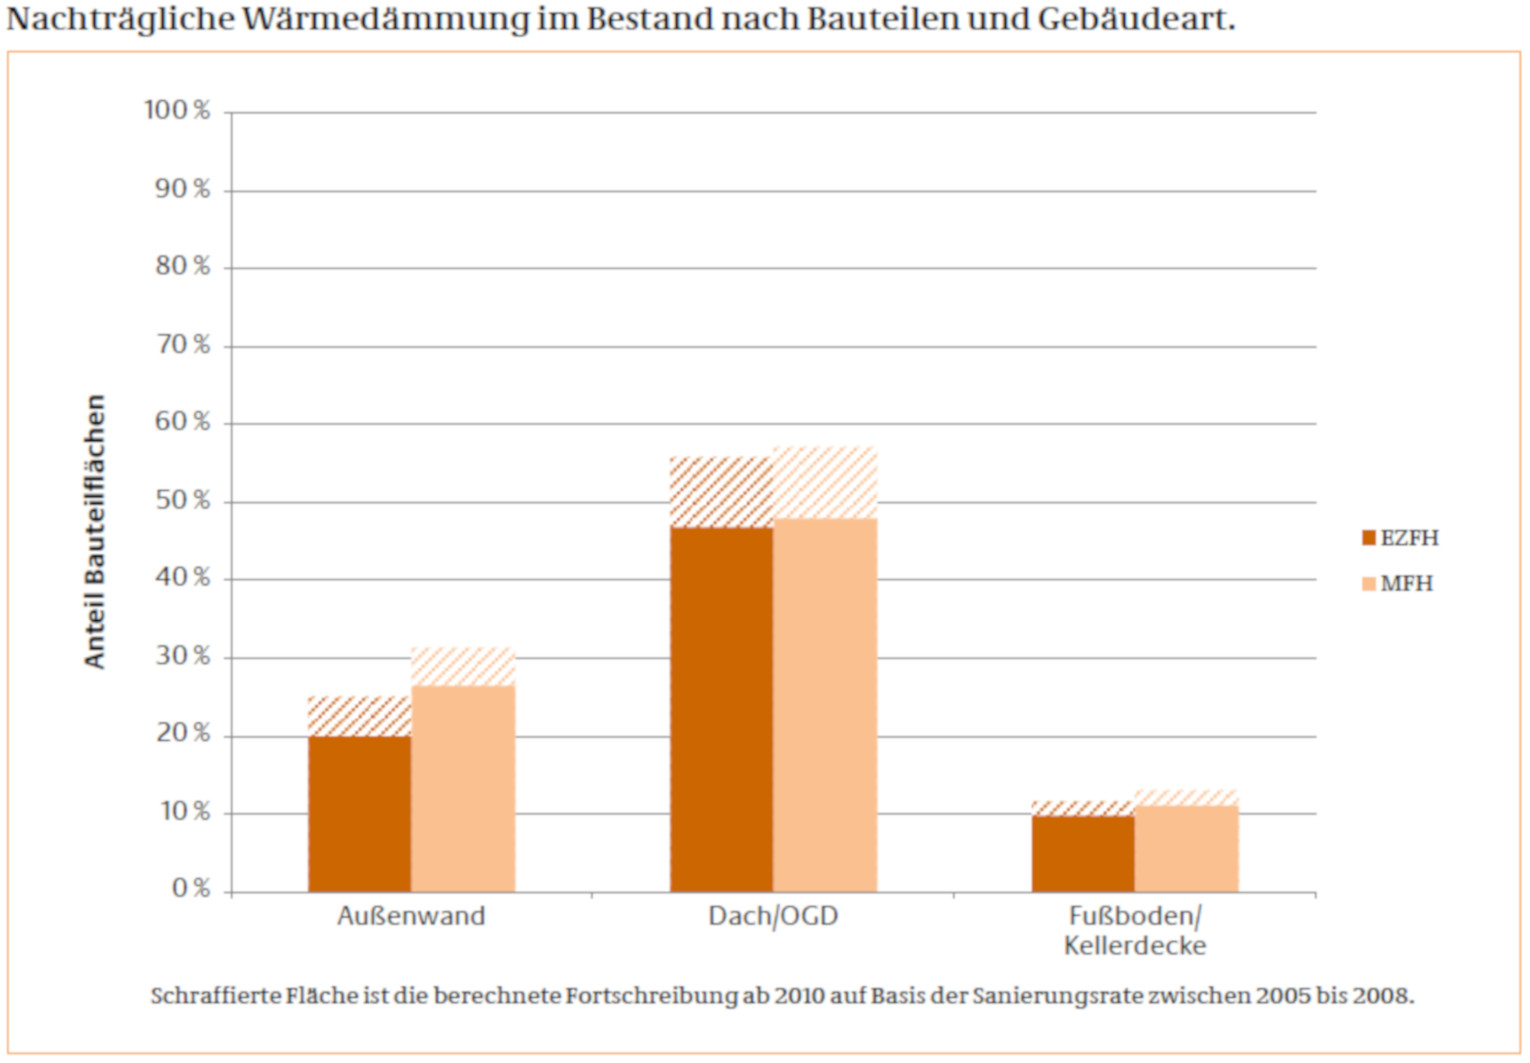
\includegraphics{Pictures/NachtraeglicheSanierung.jpg}
	\caption{Anteil der Gebäudetypen Ein- und Zweifamilienhäuser sowie Mehrfamilienhäuser mit nachträglicher Dämmung der Bauteile Außenwand, Dach/Obergeschossdecke und Fußboden/Kellerdecke \cite{Bigalke.2016}}
	\label{fig: Abbildung231} 
\end{figure}

\section{Förderprogramme zur energetischen Sanierung}
\label{sec:Sektion 24}

In Kapitel \ref{sec:Sektion 22} werden diverse Verordnungen zum besseren Wärmeschutz des deutschen Gebäudebestandes beschrieben.
Diese verkörpern Anforderungen an den Neubau oder an Einzelsanierungsmaßnahmen und nur wenige Forderungen richten sich an den Gebäudebestand.
Zur Steigerung der Wirtschaftlichkeit der energetischen Sanierungsmaßnahmen unterstützt die Bundesregierung Gebäudeeigentümer finanziell bei Maßnahmen zur Steigerung des Wärmeschutzes.

Als Beispiel eines erfolgreichen Anreizprogramms sei der flächendeckende Austausch der Einfachverglasung genannt.
Im Rahmen des Energiespar-Förderprogrammes investierte die Bundesregierung ab 1977 4,35 Milliarden Deutsche Mark zur Erneuerung von Heizungen und Fenstern \cite{EickeHenning.2011b}.
Dadurch konnte ein Anreiz zur energetischen Sanierung geschaffen werden.
Dies stellt mitunter einen Grund dafür dar, dass der Anteil der Einfachverglasung in deutschen Wohngebäuden heute nur etwa 3\,\% beträgt (s. Tabelle \ref{tab: TabelleA2}).

Es existieren verschiedene Fördermöglichkeiten, welche die Energieeffizienz der Heizungstechnik, den Einsatz erneuerbarer Energien zur Wärmeerzeugung und die energetische Ertüchtigung der Gebäudehülle subventionieren.
Die Auszahlung der öffentlichen Gelder erfolgt größtenteils durch das Bundesamt für Wirtschaft und Ausfuhrkontrolle (BAFA) und das Kreditinstitut für Wiederaufbau (KfW).
Letztere hat im Jahr 2018 insgesamt 12 Milliarden Euro an Krediten und Zuschüssen im Bereich der Energiewende für circa 220.000 Anträge an Privatkunden vergeben \cite{KfW_Report18}. 
Tabelle \ref{tab: Tabelle241} listet einige Förder- und Anreizprogramme mit den zu fördernden Technologien beziehungsweise Maßnahmen auf.

\begin{table}[H]\centering
\begin{tabular}{|l|r|r|}
\hline
\rowcolor[HTML]{C0C0C0} 
Programmbezeichnung & \multicolumn{1}{l|}{\cellcolor[HTML]{C0C0C0}Fördertyp} & \multicolumn{1}{l|}{\cellcolor[HTML]{C0C0C0}\begin{tabular}[c]{@{}l@{}}Geförderte Technologie/\\ Maßnahme\end{tabular}} \\ \hline
\begin{tabular}[c]{@{}l@{}}Erneuerbare-Energien-\\ Gesetz (EEG)\end{tabular} & Einspeisevergütung & Photovoltaik \\ \hline
\rowcolor[HTML]{EFEFEF} 
\begin{tabular}[c]{@{}l@{}}Kraft-Wärme-Kopplung- \\ Gesetz (KWKG)\end{tabular} & \begin{tabular}[c]{@{}r@{}}Einspeise-/Eigenverbrauch-\\ vergütung\end{tabular} & BHKWs \\ \hline
\begin{tabular}[c]{@{}l@{}}Mini-KWK-Zuschuss\\ (durch BAFA)\end{tabular} & Investitionszuschuss & BHKWs \\ \hline
\rowcolor[HTML]{EFEFEF} 
\begin{tabular}[c]{@{}l@{}}Anreizprogramm \\ Energieeffizienz (APEE)\end{tabular} & Investitionszuschuss & \begin{tabular}[c]{@{}r@{}}Wärmepumpen\\ Solarthermie\\ Pelletkessel\end{tabular} \\ \hline
KfW-Programm 430 & Investitionszuschuss & \begin{tabular}[c]{@{}r@{}}Sanierung von einzelnen Bauteilen \\ oder KfW-Effizienzhausstandard\end{tabular} \\ \hline
\end{tabular}
\caption{Übersicht über verschiedene Förder- und Anreizprogramme zur energetischen Verbesserung von Wohngebäuden}
\label{tab: Tabelle241}
\end{table}

%Dena Gebäudereport S. 151


